\documentclass{standalone}
\usepackage{tikz}
\usepackage{amsmath}
\begin{document}
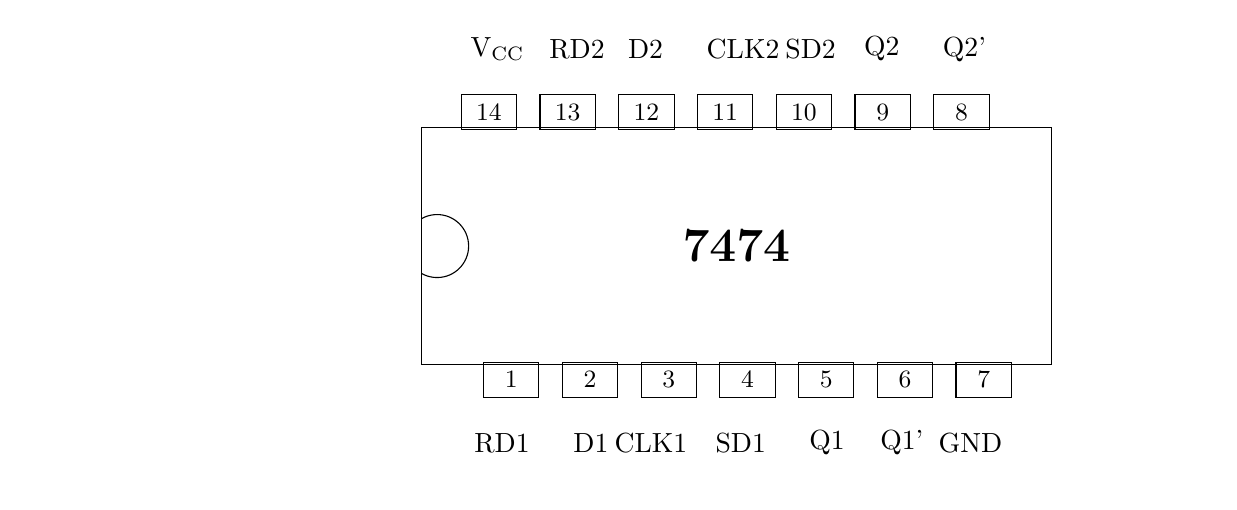
\begin{tikzpicture}[scale=1,
     pin/.style={draw,rectangle,minimum width=2em,font=\small}
     ]
   % Main trick: loop over the label numbers and then adjust their position
   % in the tikzpicture using evaluate to calculate \y=y-coordinate of pin

   \foreach \i/\desc [evaluate=\i  as \x using (\i+5 )]
      in {1/{RD1},
          2/{D1},
          3/{CLK1},
          4/{SD1},
          5/{Q1},
          6/{Q1'},
          7/{GND}}
   {
     \draw node[pin,anchor=east,rotate=360] at (\x+.5,-.2){\small$\i$};
     \node[align=right,anchor=east,rotate=360] at (\x+.5,-1){\desc};
   }
  
   \foreach \i/\desc [evaluate=\i as \x using (20-\i)]
      in {8/{Q2'},
          9/{Q2},
          10/{SD2},
          11/{CLK2},
          12/{D2},
          13/{RD2},
          14/{V$_{\text{CC}}$}}
   {
     \draw node[pin,anchor=west,rotate=360] at (\x-.5,3.2){\small$\i$};
     \node[align=right,anchor=west,rotate=360] at (\x-.5,4){\desc};
   }
   \draw
      (5,0.8)--(5,3)--(5,3)--(13,3)--(13,3)
             --(13,0.8)--(13,0)--(5,0)--cycle;
    \begin{scope}         
    \clip (15,.5) rectangle (5,2);         
   \draw(5.2,1.5)circle[radius=0.4];
   \end{scope}
   \begin{scope}
   \clip (0,-1.5) rectangle (1.5,1.5);
    \draw (2,) circle(6.5);
\end{scope}

   \node at (9,1.5){\textbf{\LARGE{7474}}};
 \end{tikzpicture}
\end{document}



